\documentclass[
  shownotes,
  xcolor={svgnames},
  hyperref={colorlinks,citecolor=DarkBlue,linkcolor=DarkRed,urlcolor=DarkBlue}
  , aspectratio=169]{beamer}
\usepackage{animate}
\usepackage{amsmath}
\usepackage{amsfonts}
\usepackage{amssymb}
\usepackage{pifont}
\usepackage{mathpazo}
%\usepackage{xcolor}
\usepackage{multimedia}
\usepackage{fancybox}
\usepackage[para]{threeparttable}
\usepackage{multirow}
\setcounter{MaxMatrixCols}{30}
\usepackage{subcaption}
\usepackage{graphicx}
\usepackage{lscape}
\usepackage[compatibility=false,font=small]{caption}
\usepackage{booktabs}
\usepackage{ragged2e}
\usepackage{chronosys}
\usepackage{appendixnumberbeamer}
\usepackage{animate}
\setbeamertemplate{caption}[numbered]
\usepackage{color}
%\usepackage{times}
\usepackage{tikz}
\usepackage{comment} %to comment
%% BibTeX settings
\usepackage{natbib}
\bibliographystyle{apalike}
\bibpunct{(}{)}{,}{a}{,}{,}
\setbeamertemplate{bibliography item}{[\theenumiv]}

% Defines columns for bespoke tables
\usepackage{array}
\newcolumntype{L}[1]{>{\raggedright\let\newline\\\arraybackslash\hspace{0pt}}m{#1}}
\newcolumntype{C}[1]{>{\centering\let\newline\\\arraybackslash\hspace{0pt}}m{#1}}
\newcolumntype{R}[1]{>{\raggedleft\let\newline\\\arraybackslash\hspace{0pt}}m{#1}}


\usepackage{xfrac}


\usepackage{multicol}
\setlength{\columnsep}{0.5cm}

% Theme and colors
\usetheme{Boadilla}

% I use steel blue and a custom color palette. This defines it.
\definecolor{andesred}{HTML}{af2433}

% Other options
\providecommand{\U}[1]{\protect\rule{.1in}{.1in}}
\usefonttheme{serif}
\setbeamertemplate{itemize items}[default]
\setbeamertemplate{enumerate items}[square]
\setbeamertemplate{section in toc}[circle]

\makeatletter

\definecolor{mybackground}{HTML}{82CAFA}
\definecolor{myforeground}{HTML}{0000A0}

\setbeamercolor{normal text}{fg=black,bg=white}
\setbeamercolor{alerted text}{fg=red}
\setbeamercolor{example text}{fg=black}

\setbeamercolor{background canvas}{fg=myforeground, bg=white}
\setbeamercolor{background}{fg=myforeground, bg=mybackground}

\setbeamercolor{palette primary}{fg=black, bg=gray!30!white}
\setbeamercolor{palette secondary}{fg=black, bg=gray!20!white}
\setbeamercolor{palette tertiary}{fg=white, bg=andesred}

\setbeamercolor{frametitle}{fg=andesred}
\setbeamercolor{title}{fg=andesred}
\setbeamercolor{block title}{fg=andesred}
\setbeamercolor{itemize item}{fg=andesred}
\setbeamercolor{itemize subitem}{fg=andesred}
\setbeamercolor{itemize subsubitem}{fg=andesred}
\setbeamercolor{enumerate item}{fg=andesred}
\setbeamercolor{item projected}{bg=gray!30!white,fg=andesred}
\setbeamercolor{enumerate subitem}{fg=andesred}
\setbeamercolor{section number projected}{bg=gray!30!white,fg=andesred}
\setbeamercolor{section in toc}{fg=andesred}
\setbeamercolor{caption name}{fg=andesred}
\setbeamercolor{button}{bg=gray!30!white,fg=andesred}


\usepackage{fancyvrb}
\newcommand{\VerbBar}{|}
\newcommand{\VERB}{\Verb[commandchars=\\\{\}]}
\DefineVerbatimEnvironment{Highlighting}{Verbatim}{commandchars=\\\{\}}
% Add ',fontsize=\small' for more characters per line
\usepackage{framed}
\definecolor{shadecolor}{RGB}{248,248,248}
\newenvironment{Shaded}{\begin{snugshade}}{\end{snugshade}}
\newcommand{\AlertTok}[1]{\textcolor[rgb]{0.94,0.16,0.16}{#1}}
\newcommand{\AnnotationTok}[1]{\textcolor[rgb]{0.56,0.35,0.01}{\textbf{\textit{#1}}}}
\newcommand{\AttributeTok}[1]{\textcolor[rgb]{0.77,0.63,0.00}{#1}}
\newcommand{\BaseNTok}[1]{\textcolor[rgb]{0.00,0.00,0.81}{#1}}
\newcommand{\BuiltInTok}[1]{#1}
\newcommand{\CharTok}[1]{\textcolor[rgb]{0.31,0.60,0.02}{#1}}
\newcommand{\CommentTok}[1]{\textcolor[rgb]{0.56,0.35,0.01}{\textit{#1}}}
\newcommand{\CommentVarTok}[1]{\textcolor[rgb]{0.56,0.35,0.01}{\textbf{\textit{#1}}}}
\newcommand{\ConstantTok}[1]{\textcolor[rgb]{0.00,0.00,0.00}{#1}}
\newcommand{\ControlFlowTok}[1]{\textcolor[rgb]{0.13,0.29,0.53}{\textbf{#1}}}
\newcommand{\DataTypeTok}[1]{\textcolor[rgb]{0.13,0.29,0.53}{#1}}
\newcommand{\DecValTok}[1]{\textcolor[rgb]{0.00,0.00,0.81}{#1}}
\newcommand{\DocumentationTok}[1]{\textcolor[rgb]{0.56,0.35,0.01}{\textbf{\textit{#1}}}}
\newcommand{\ErrorTok}[1]{\textcolor[rgb]{0.64,0.00,0.00}{\textbf{#1}}}
\newcommand{\ExtensionTok}[1]{#1}
\newcommand{\FloatTok}[1]{\textcolor[rgb]{0.00,0.00,0.81}{#1}}
\newcommand{\FunctionTok}[1]{\textcolor[rgb]{0.00,0.00,0.00}{#1}}
\newcommand{\ImportTok}[1]{#1}
\newcommand{\InformationTok}[1]{\textcolor[rgb]{0.56,0.35,0.01}{\textbf{\textit{#1}}}}
\newcommand{\KeywordTok}[1]{\textcolor[rgb]{0.13,0.29,0.53}{\textbf{#1}}}
\newcommand{\NormalTok}[1]{#1}
\newcommand{\OperatorTok}[1]{\textcolor[rgb]{0.81,0.36,0.00}{\textbf{#1}}}
\newcommand{\OtherTok}[1]{\textcolor[rgb]{0.56,0.35,0.01}{#1}}
\newcommand{\PreprocessorTok}[1]{\textcolor[rgb]{0.56,0.35,0.01}{\textit{#1}}}
\newcommand{\RegionMarkerTok}[1]{#1}
\newcommand{\SpecialCharTok}[1]{\textcolor[rgb]{0.00,0.00,0.00}{#1}}
\newcommand{\SpecialStringTok}[1]{\textcolor[rgb]{0.31,0.60,0.02}{#1}}
\newcommand{\StringTok}[1]{\textcolor[rgb]{0.31,0.60,0.02}{#1}}
\newcommand{\VariableTok}[1]{\textcolor[rgb]{0.00,0.00,0.00}{#1}}
\newcommand{\VerbatimStringTok}[1]{\textcolor[rgb]{0.31,0.60,0.02}{#1}}
\newcommand{\WarningTok}[1]{\textcolor[rgb]{0.56,0.35,0.01}{\textbf{\textit{#1}}}}
\usepackage{graphicx}
\makeatletter

\usepackage{tikz}
% Tikz settings optimized for causal graphs.
\usetikzlibrary{shapes,decorations,arrows,calc,arrows.meta,fit,positioning}
\tikzset{
    -Latex,auto,node distance =1 cm and 1 cm,semithick,
    state/.style ={ellipse, draw, minimum width = 0.7 cm},
    point/.style = {circle, draw, inner sep=0.04cm,fill,node contents={}},
    bidirected/.style={Latex-Latex,dashed},
    el/.style = {inner sep=2pt, align=left, sloped}
}


\makeatother






%%%%%%%%%%%%%%% BEGINS DOCUMENT %%%%%%%%%%%%%%%%%%

\begin{document}

\title[Lecture 7]{Lecture 7: \\  Bayesian Estimation Methods}
\subtitle{Big Data and Machine Learning for Applied Economics \\ Econ 4676}
\date{\today}

\author[Sarmiento-Barbieri]{Ignacio Sarmiento-Barbieri}
\institute[Uniandes]{Universidad de los Andes}


\begin{frame}[noframenumbering]
\maketitle
\end{frame}

%%%%%%%%%%%%%%%%%%%%%%%%%%%%%%%%%%%


%----------------------------------------------------------------------%
\begin{frame}
\frametitle{Recap}

\begin{itemize} 

    \item OLS      
    \bigskip
    \item MLE
    \bigskip
    \item Computation
    
  
\end{itemize}
\end{frame}

%----------------------------------------------------------------------%

\begin{frame}
\frametitle{Agenda}

\tableofcontents


\end{frame}





%----------------------------------------------------------------------%
\section{The Bayesian Approach}
%----------------------------------------------------------------------%
\begin{frame}[fragile]
\frametitle{The Bayesian Approach}

\begin{itemize}
\item We've been living in a ``frequentist'' world
\medskip
\item Observe the data
\medskip
\item Impose some assumptions on the data
\begin{align}
X_1,X_2,\dots,X_n \sim_{iid} f(X|\theta)
\end{align}
\medskip
\item The parameter $\theta$ is thought to be unknown
\end{itemize}
\end{frame}
%----------------------------------------------------------------------%
\begin{frame}[fragile]
\frametitle{The Bayesian Approach}

\begin{itemize}
\item What happens if we have a prior belief of $\theta$?
\medskip
\item How can we incorporate this information?
\medskip
\item Bayesian Statistics gives us a framework to do it a systematic way

\end{itemize}


\end{frame}
%----------------------------------------------------------------------% 
\section{A Simple Covid Example}
%----------------------------------------------------------------------%
\begin{frame}[fragile]
\frametitle{A Simple Covid Example}
\begin{itemize}
\item Suppose we are interested in the prevalence of COVID in a small city. 
\medskip
\item The higher the prevalence, the more public health precautions we would recommend be put into place. 
\medskip
\item A small random sample of 20 individuals from the city will be checked for the presence of the virus.
\medskip
\item Interest is in $\theta$, the fraction of infected individuals in the city. 
\medskip
\item $X$ records the total number of people in the sample who are infected. Before the sample is obtained the number of infected individuals in the sample is unknown.
\end{itemize}


\end{frame}

%----------------------------------------------------------------------%
\begin{frame}[fragile]
\frametitle{A Simple Covid Example}

\begin{itemize}
\footnotesize
 \item If the value of $\theta$ were known, a reasonable sampling model would be
 \begin{align}
 X|\theta \sim Binomial(20,\theta)
 \end{align}

 \item Suppose we observe the following data, this is consistent with $\theta=.2$
 \begin{figure}[H] \centering
  \centering
  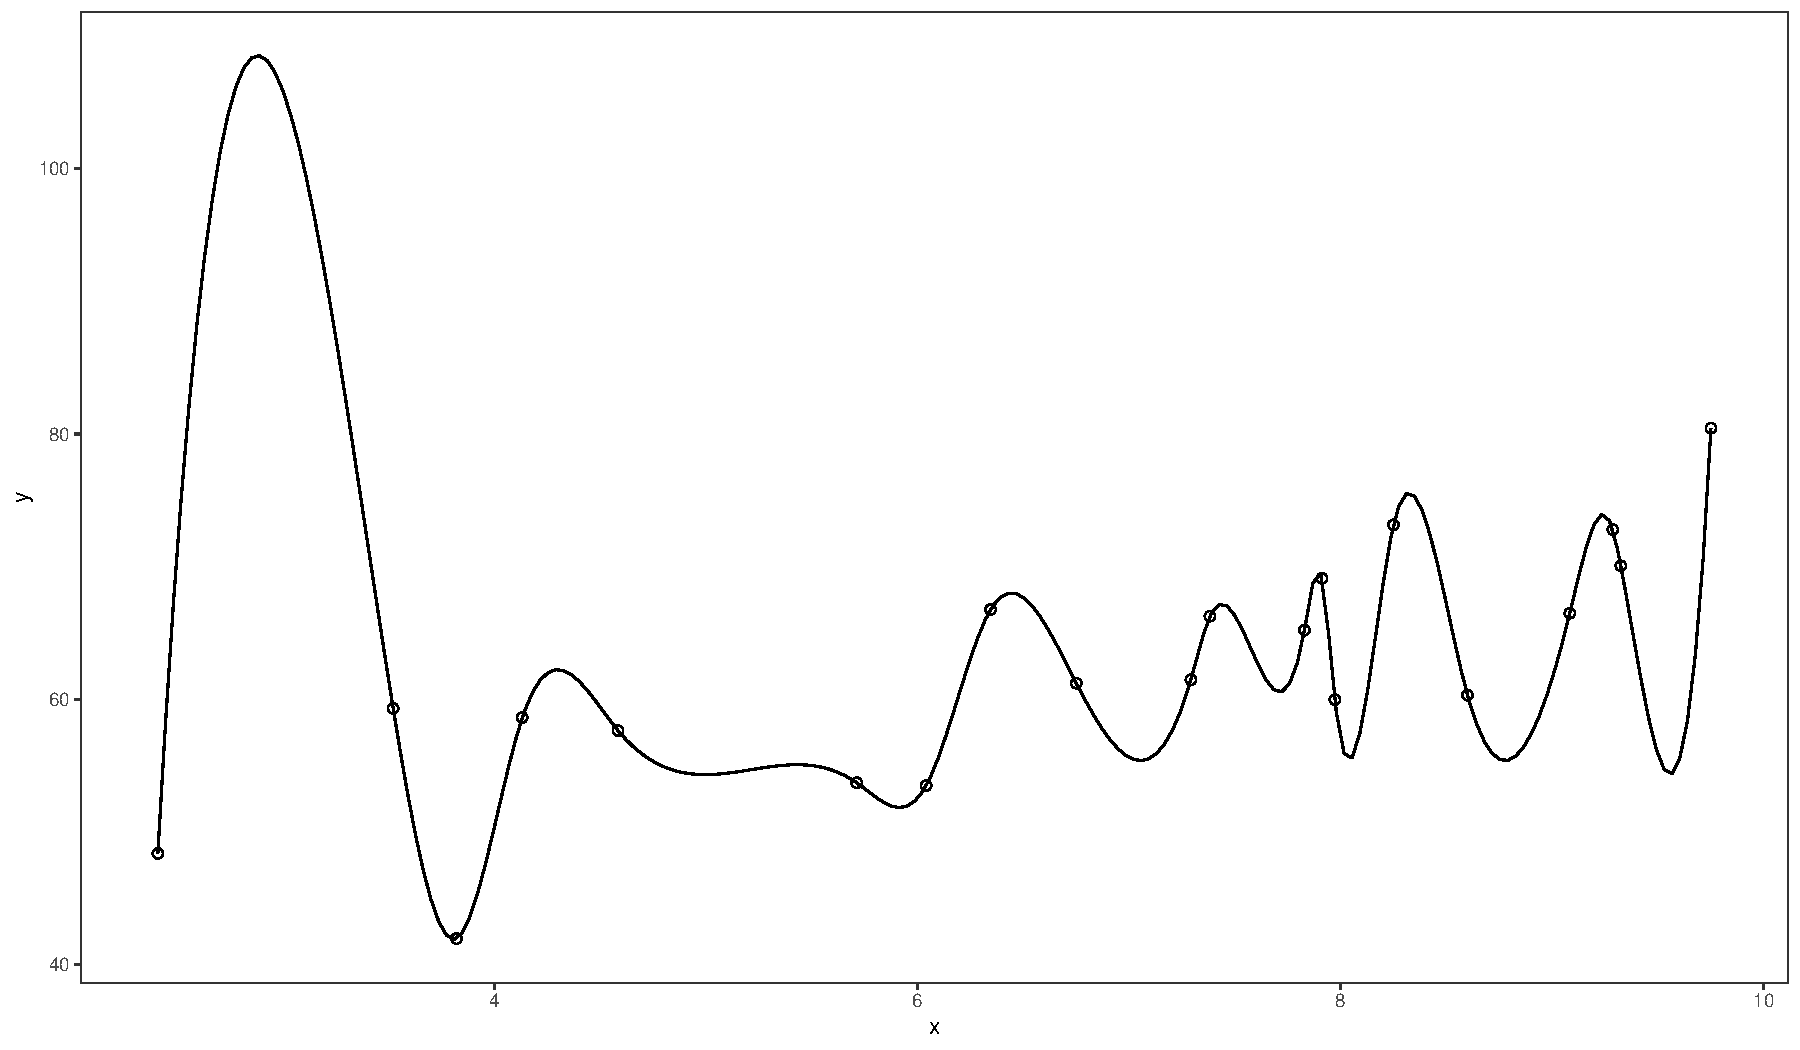
\includegraphics[scale=0.25]{figures/fig_1c}
  \\
  \tiny 
\end{figure}

\tiny
 \begin{align}
 Pr(X=x)= \binom{n}{x}\theta^x(1-\theta)^{n-x} \\
 Pr(X=0)= \binom{20}{0}0.2^0(1-0.2)^{20-0} \approx 0.01
 \end{align}
\end{itemize}


\end{frame}
%----------------------------------------------------------------------%
\begin{frame}[fragile]
\frametitle{A Simple Covid Example}
\framesubtitle{Prior distribution}

\begin{itemize}
\item Other studies from various parts of the country indicate that the infection rate in comparable cities ranges from about 0.05 to 0.20, with an average prevalence of 0.10.

\medskip
\item How can we incorporate this information?
\medskip

\item Bayes Theorem to the rescue
\end{itemize}



\end{frame}
%----------------------------------------------------------------------%
\begin{frame}[fragile]
\frametitle{Bayes Theorem}
For this updating we use {\it Bayes Theorem}

\bigskip
\begin{align}
\pi (\theta|X)=\frac{f(X|\theta)p(\theta)}{m(X)}
\end{align}

\bigskip
with $m(X)$ is the marginal distribution of $X$, i.e.

\begin{align}
m(X)=\int f(X|\theta)p(\theta)d\theta
\end{align}

It is important to note that Bayes' theorem  does not tell us what our beliefs should be, it tells us how they should change after seeing new information.
\end{frame}
%----------------------------------------------------------------------%
\begin{frame}[fragile]
\frametitle{A Simple Covid Example}
\framesubtitle{Prior distribution}

\begin{itemize}
\item We can characterize our prior ($p(\theta)$) with a Beta distribution 
\end{itemize}


\begin{align}
\theta \sim Beta(a,b)
\end{align}
where the density of a Beta takes the form of

\begin{align}
p(\theta)=\frac{\Gamma\left(a+b\right)}{\Gamma\left(a\right)\Gamma\left(b\right)}\theta^{a-1}\left(1-\theta\right)^{b-1}
\end{align}

\end{frame}
%----------------------------------------------------------------------%
\begin{frame}[fragile]
\frametitle{A Simple Covid Example}
\framesubtitle{Prior distribution}

For now let, $a=2$ and $b=20$. 

 \begin{figure}[H] \centering
  \centering
  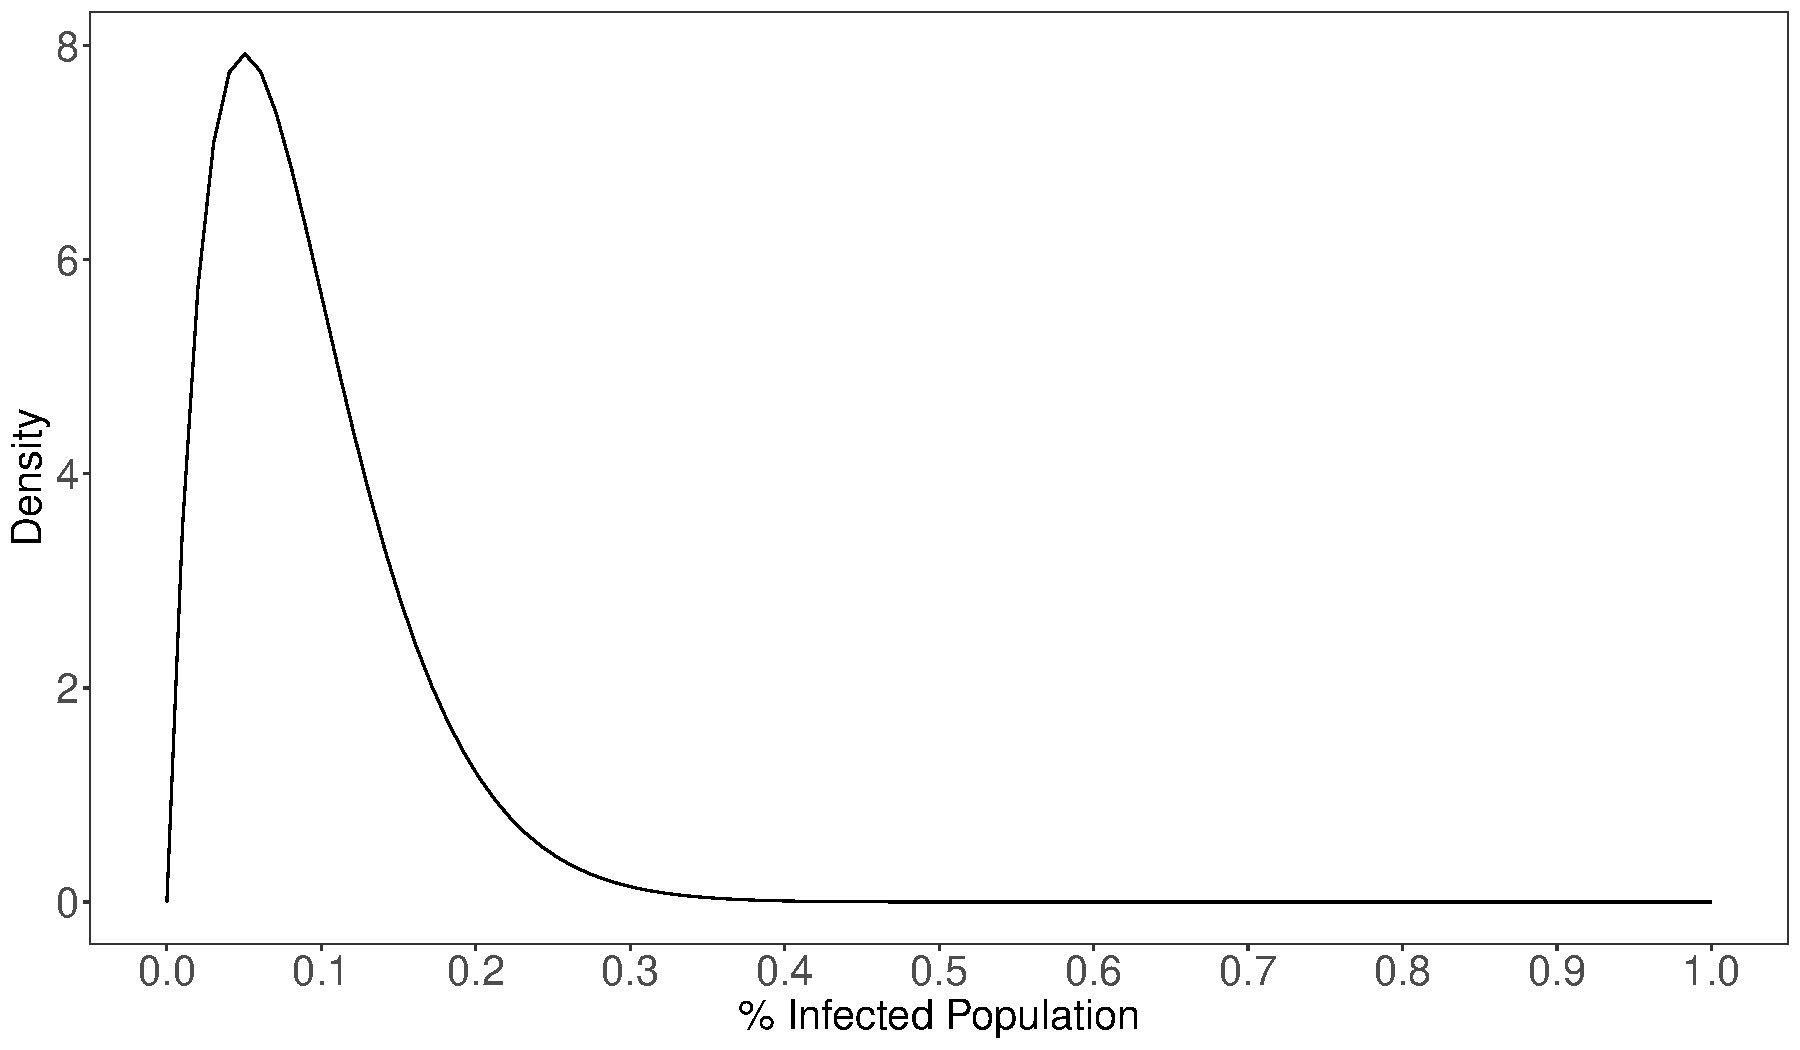
\includegraphics[scale=0.25]{figures/fig_beta}
  \\
  \tiny 
\end{figure}

\begin{align}
E(\theta) =\frac{a}{a+b} =0.09 \\
Pr(0.05 < \theta < 0.20) = 0.66
\end{align}

\end{frame}
%----------------------------------------------------------------------%
\begin{frame}[fragile]
\frametitle{A Simple Covid Example}
\framesubtitle{Posterior distribution}

\begin{align}
\pi(\theta|X) &= \frac{f(X|\theta)p(\theta)}{m(X)} 
\end{align}


\begin{align}
\pi(\theta|X) &=  \binom{n}{x}\theta^x(1-\theta)^{n-x} \times\frac{\Gamma(a+b)}{\Gamma(a)\Gamma(b)}\theta^{a-1}(1-\theta)^{b-1}  \frac{1}{m(x)}
\end{align}

The marginal

\begin{scriptsize}
\begin{align}
m(x) &= \int f(X|\theta)p(\theta)d\theta \\
 &= \int_0^1 \binom{n}{x}\theta^x(1-\theta)^{n-x} \times\frac{\Gamma(a+b)}{\Gamma(a)\Gamma(b)}\theta^{a-1}(1-\theta)^{b-1}  d\theta \\
 &= \binom{n}{x} \frac{\Gamma(a+b)}{\Gamma(a)\Gamma(b)} \int_0^1 \theta^{x+a-1}(1-\theta)^{n-x+b-1}  d\theta 
\end{align}
\end{scriptsize}
\end{frame}
%----------------------------------------------------------------------%
\begin{frame}[fragile]
\frametitle{A Simple Covid Example}
\framesubtitle{Posterior distribution}
The marginal (cont)

\begin{scriptsize}
\begin{align}
%m(x) &= \int f(X|\theta)p(\theta)d\theta \\
 %&= \int_0^1 \binom{n}{x}\theta^x(1-\theta)^{n-x} \times\frac{\Gamma(a+b)}{\Gamma(a)\Gamma(b)}\theta^{a-1}(1-\theta)^{b-1}  d\theta \\
 %&= \binom{n}{x} \frac{\Gamma(a+b)}{\Gamma(a)\Gamma(b)} \int_0^1 \theta^{x+a-1}(1-\theta)^{n-x+b-1}  d\theta \\
 m(x) &= \binom{n}{x} \frac{\Gamma(a+b)}{\Gamma(a)\Gamma(b)}  \frac{\Gamma(a+x)\Gamma(b+n-x)}{\Gamma(a+b+n)} \int_0^1  \frac{\Gamma(a+b+n)}{\Gamma(a+x)\Gamma(b+n-x)} \theta^{x+a-1}(1-\theta)^{n-x+b-1}  d\theta \\
 &= \binom{n}{x} \frac{\Gamma(a+b)}{\Gamma(a)\Gamma(b)}  \frac{\Gamma(a+x)\Gamma(b+n-x)}{\Gamma(a+b+n)}
\end{align}
\end{scriptsize}

The posterior
\begin{align}
\pi(\theta|X) &=  \frac{\Gamma(a+b+n)}{\Gamma(a+x)\Gamma(b+n-x)} \theta^{x+a-1}(1-\theta)^{n-x+b-1}  \\
              &\sim Beta(a+x,b+n-x)
\end{align}

\end{frame}
%----------------------------------------------------------------------%
\begin{frame}[fragile]
\frametitle{A Simple Covid Example}
With the posterior we can calculate then any moment of the posterior distribution. For example suppose that for our study none of the sample of individuals is infected (x=0). Then the posterior is 

\medskip
\begin{align}
\pi(\theta|X=0) &\sim Beta(2,40)
\end{align}

\medskip
$a= 2$, $b=20$, $n=20$. Then

\medskip

\begin{align}
E(\theta|X=0)  &= 0.048 
\end{align}

\end{frame}
%----------------------------------------------------------------------%
\begin{frame}[fragile]
\frametitle{A Simple Covid Example}

How did we get there?
\medskip
\begin{align}
E(\theta|X=0)  &= \frac{a+x}{a+b+n} \\
               &= \frac{n}{a+b+n} \frac{x}{n} + \frac{a+b}{a+b+n} \frac{a}{a+b}  \\
               &= \frac{n}{a+b+n} \bar x + \frac{a+b}{a+b+n} \theta_{prior}  \\
               &= \frac{n}{a+b+n} 0 + \frac{a+b}{a+b+n} \frac{2}{22}  \\
 &= 0.048 
\end{align}

Recall that $a= 2$, $b=20$, $n=20$

\end{frame}
%----------------------------------------------------------------------%
\begin{frame}[fragile]
\frametitle{A Simple Covid Example}

Since we have the full distribution we could calculate for example:
\begin{align}
mode(\theta|X) = 0.025 \\
Pr(\theta<0.20|X=0) &= 0.998
\end{align}

\begin{figure}[H] \centering
  \centering
  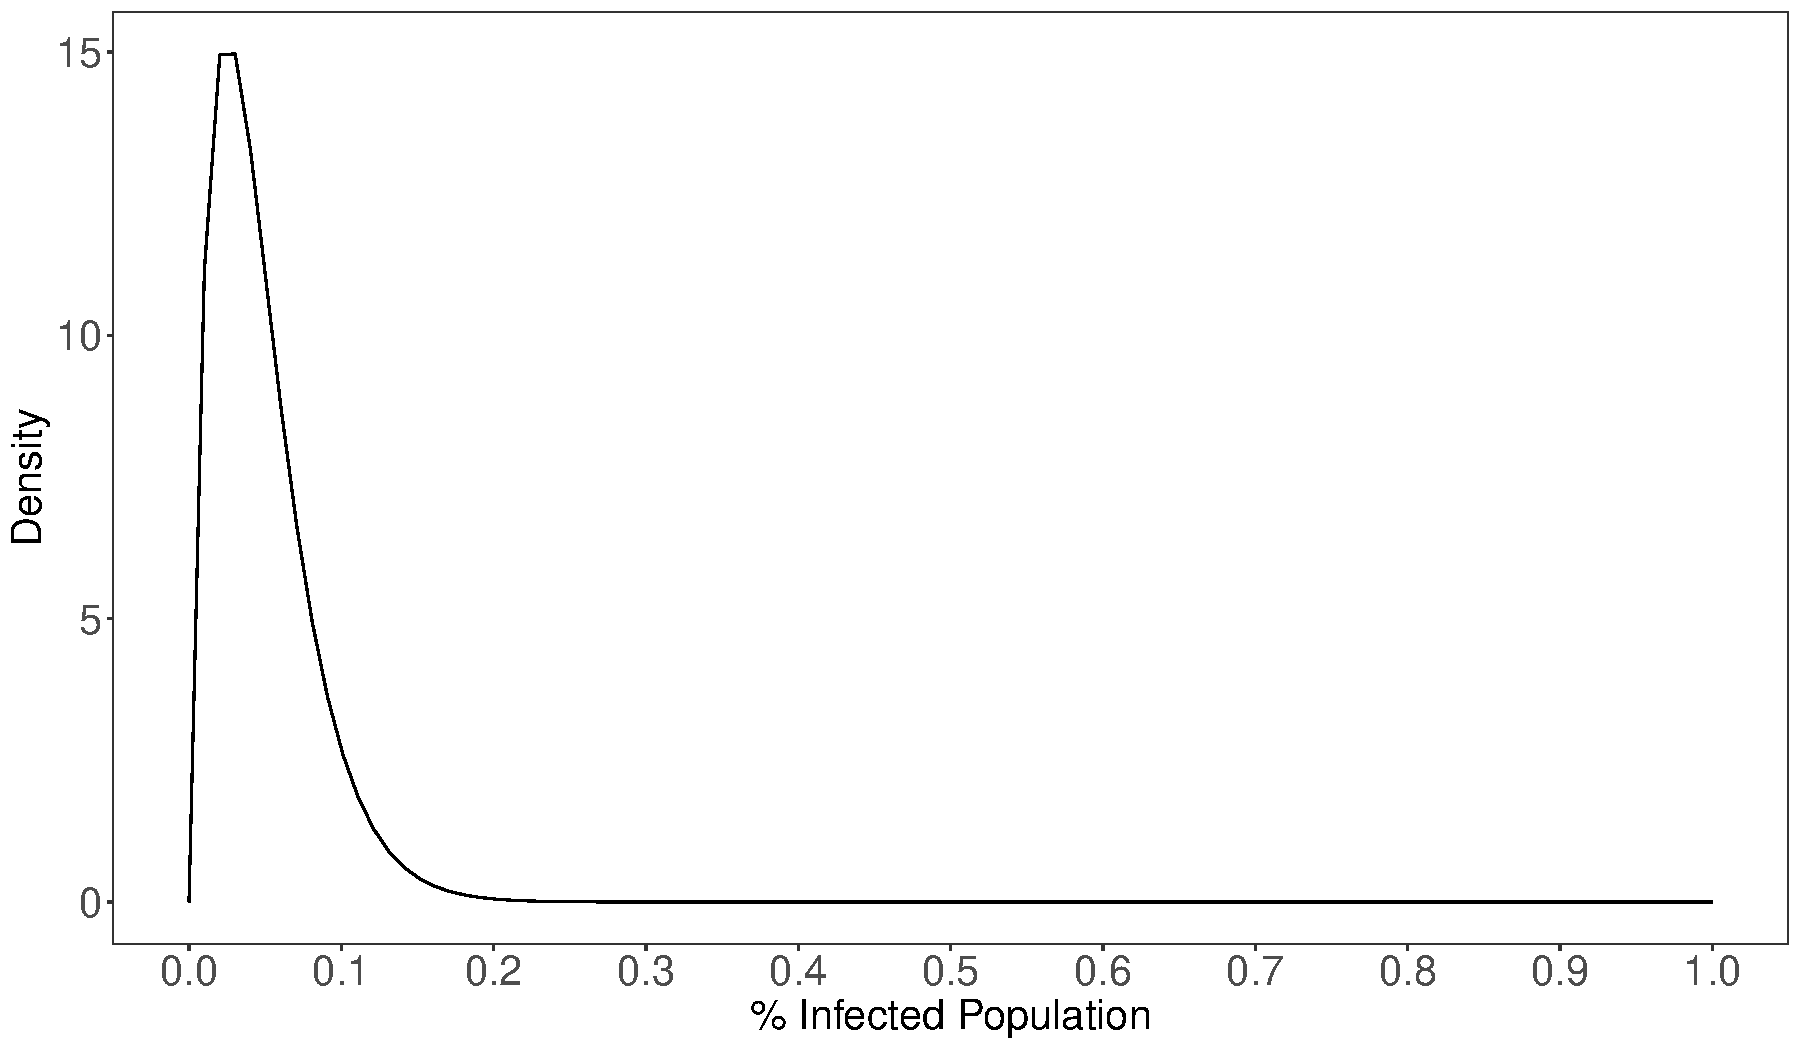
\includegraphics[scale=0.25]{figures/fig_2}
  \\
  \tiny 
\end{figure}


\end{frame}

%----------------------------------------------------------------------%
\begin{frame}[fragile]
\frametitle{Bayesian Estimation}


\begin{itemize}
\item The Bayesian approach to stats is fundamentally different from the classical approach we have been taking
\medskip
\item In the classical approach, the parameter $\theta$ is thought to be an unknown, but fixed quantity, e.g., $X_i\sim f(\theta)$
\medskip
\item In the Bayesian approach $\theta$ is considered to be a quantity whose variation can be described by a probability distribution  ({\it prior distribution})
\medskip
\item Then a sample is taken from a population indexed by $\theta$ and the prior is updated with this sample
\medskip
\item The resulting updated prior is the {\it posterior distribution}
\end{itemize}
\end{frame}

%----------------------------------------------------------------------%
\begin{frame}[fragile]
\frametitle{Conjugate Priors}

{\bf Definition}
Let $\mathcal{F}$ denote the class of densities $f(x|\theta)$. A class $\mathcal{C}$ of prior distributions is a conjugate family for $\mathcal{F}$ if the posterior distribution is in the class $\mathcal{C}$ for all $f\in\mathcal{F}$, all priors in $\mathcal{C}$, and all $x\in X$

\medskip

 

{\footnotesize For example:}

\begin{itemize}
  \footnotesize
  \item $X\sim D(\theta)$ and $\theta \sim P(\lambda)$ $\rightarrow$ $\theta|X \sim P(\lambda')$
  \item the normal distribution is a conjugate for the normal family \\
   $X\sim N(\mu,\sigma)$ and $\theta \sim N(\mu_0,\sigma_0)$ $\rightarrow$ $\theta|X \sim N(\mu',\sigma')$
  \item the beta distribution for the binomial family \\ 
  $X\sim Bernoulli(\theta)$ and $\theta \sim Beta(a,b)$ $\rightarrow$ $\theta|X \sim Beta(a',b')$
  
\end{itemize}

\medskip
\footnotesize
Good and bad news:
\begin{itemize}
\item Nice because gives us a closed form for the posterior. However, whether a conjugate family is a reasonable choice is left to you!
\item Downside, if we choose another families, then these results are no longer available. Then we have to use sampling-based methods ( Gibbs Sampler, MCMC, etc)
\end{itemize}


\end{frame}
%----------------------------------------------------------------------%
\begin{frame}[fragile]
\frametitle{Bayesian Linear Regression}

Consider

\begin{align}
y_i= \beta x_i+u_i\,\,\,u_i \sim_{iid} N(0,\sigma^2)
\end{align}

The likelihood function is

\begin{align}
f(y|\beta,\sigma,x)=\Pi_{i=1}^n\frac{1}{(\sqrt{2\pi\sigma^2})}e^{-\frac{1}{2\sigma^2}(y_i-\beta x_i)^2}
\end{align}
Now consider that the prior for $\beta$ is $N(\beta_0,\tau^2)$

\begin{align}
p(\beta)=\frac{1}{\sqrt{2\pi\tau^2}}e^{-\frac{1}{2\tau^2}{(\beta-\beta_0)^2}}
\end{align}

\end{frame}
%----------------------------------------------------------------------%
\begin{frame}[fragile]
\frametitle{Bayesian Linear Regression}
The Posterior distribution then 

\begin{align}
\pi (\beta|y,x) &= \frac{f(y,x|\beta)p(\beta)}{m(y,x)} \\
&= \frac{f(y|x,\beta)f(x|\beta)p(\beta)}{m(y,x)}
\end{align}

by assumption $f(x|\beta)=f(x)$

\begin{align}
&= f(y|x,\beta)p(\beta)\frac{f(x)}{m(y,x)}
\end{align}
\begin{align}
\propto f(y|x,\beta)p(\beta)
\end{align}

\end{frame}
%----------------------------------------------------------------------%
\begin{frame}[fragile]
\frametitle{Bayesian Linear Regression (Detour)}
{\bf Useful Result:} \\

\bigskip
Suppose a density of a random variable $\theta$ is proportional to

\begin{align}
  exp\left(\frac{-1}{2}(A\theta^2+B\theta)\right)
\end{align}

Then $\theta\sim N(m,V)$ where
\begin{align}
m=\frac{-1B}{2A} \,\,\,\,\,\, V=\frac{1}{A}
\end{align}


\end{frame}
%----------------------------------------------------------------------%
\begin{frame}[fragile]
\frametitle{Bayesian Linear Regression (we are back)}
\framesubtitle{$\sigma^2$ is known}

\begin{align}
P(\beta|y,X) \propto \left(\frac{1}{\sqrt{2\pi\sigma^2}}\right)^n exp\left(\frac{-1}{2\sigma^2}\sum(y_i-\beta x_i)^2\right)exp\left(\frac{-1}{2\tau^2}(\beta-\beta_0)^2\right)
\end{align}


\begin{align}
\propto  exp \left[ \frac{-1}{2} \left(\frac{1}{\sigma^2}\sum(y_i-\beta x_i)^2 + \frac{-1}{\tau^2}(\beta-\beta_0)^2\right)\right]
\end{align}

\end{frame}
%----------------------------------------------------------------------%
\begin{frame}[fragile]
\frametitle{Bayesian Linear Regression (we are back)}

Using the previous detour

\begin{align}
A= \frac{1}{\sigma^2}\sum x_i^2 +\frac{1}{\tau^2}
\end{align}
\medskip
\begin{align}
B= -2 \frac{1}{\sigma^2}\sum y_i x_i +\frac{1}{\tau^2} \beta_0
\end{align}

Then $\beta\sim N(m,V)$ with

\begin{align}
m=\frac{\frac{1}{\sigma^2}\sum y_i x_i +\frac{1}{\tau^2} \beta_0}{(\frac{1}{\sigma^2}\sum x_i^2 +\frac{1}{\tau^2})}
\end{align}

\begin{align}
 V=\frac{1}{A}
\end{align}


\end{frame}

%----------------------------------------------------------------------%
\begin{frame}[fragile]
\frametitle{Bayesian Linear Regression (we are back)}

\begin{align}
m=\left(\frac{\frac{\sum x_i^2}{\sigma^2}}{\frac{\sum x_i^2}{\sigma^2}+\frac{1}{\tau^2}}\right)\frac{\sum x_iy_i}{\sum x_i^2} + \left(\frac{\frac{1}{\tau^2}}{\frac{\sum x_i^2}{\sigma^2}+\frac{1}{\tau^2}}\right)\beta_0
\end{align}

\medskip

\begin{align}
m = \omega \hat \beta_{MLE} + (1-\omega) \beta_0
\end{align}

Remarks 

\begin{itemize}
  \item If prior belief is strong $\tau \downarrow 0 \rightarrow \omega \downarrow 0 \implies m=\beta_0$ 
  \item If prior belief is weak $\tau \uparrow \infty \rightarrow \omega \uparrow 1 \implies m=\beta_{MLE}$ 

\end{itemize}

\end{frame}


%----------------------------------------------------------------------%
\begin{frame}
\frametitle{Review \& Next Steps}
  
  \begin{itemize} 
    
    
    \item Bayesian Estimation
  \bigskip  

  
  \item  {\bf Next Class:} Cont. Bayesian Stats.
  
  
  \end{itemize}


\end{frame}


%----------------------------------------------------------------------%

\section{Further Readings}
%----------------------------------------------------------------------%
\begin{frame}
\frametitle{Further Readings}

\begin{itemize}
  \item Casella, G., \& Berger, R. L. (2002). Statistical inference (Vol. 2, pp. 337-472). Pacific Grove, CA: Duxbury. Chapter 7
  \medskip
  \item Hoff, P. D. (2009). A first course in Bayesian statistical methods (Vol. 580). New York: Springer.
  \medskip
  
  
  
\end{itemize}

\end{frame}

%----------------------------------------------------------------------%

\end{document}

%----------------------------------------------------------------------%
%----------------------------------------------------------------------%

